\documentclass[a4paper,10pt]{paper}

\usepackage[utf8]{inputenc}
\usepackage{graphicx}
\usepackage{amsmath}

\begin{document}

\title{Satogaeri}
\author{Markus Leitner}
\maketitle 
\tableofcontents

\section{Introduction}



\section{Satogaeri}
Satogaeri is a logic puzzle published by the Japanese company Nikoli Co.m Ltd. in 2002. Satogaeri only made a booklet appearance in Nikoli Vol. 99, Vol. 100 and Vol. 101. However it got revived on nikoli.com in 2013.

\subsection{Rules}
The official rules from Nikoi state:

\begin{enumerate}
  \item The areas enclosed by bold lines, are called "Countries." Move the circles, vertically or horizontally, so each country contains only one circle.
  \item The numbers in the circles indicate how many cells they have to pass through. Circles without numbers may move any distance, but some of them do not move.
  \item The circles cannot cross the tracks of other circles and cannot go over other circles. 
\end{enumerate}
And additionally the 4th rule, which counts for every logic puzzle:
\begin{enumerate}
  \item[4] A puzzle only has one solution.
\end{enumerate}

\begin{figure}
  \centering
  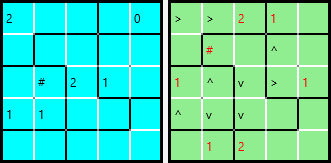
\includegraphics[scale=1]{Pictures/sample_small.png} 
  \caption{Small sample puzzle with its solution}
  \label{fig:sample_small}
\end{figure}

Handcrafted puzzles tend to have a mirrored country-layout either vertically, horizontally or both as can be seen in Figure~\ref{fig:sample_small}. Numberless Circles are here referred to as '\#'.

\section{Satisfiability Modulo Theories}
Before we can go on and talk about how to solve Satogaeri problems we first have to look intt Satisfiability Modulo Theories (SMT) for this was used to create the solver and the generator.

SMT can be seen as an enhancement of the traditional Satisfiability (SAT) solving. In SAT solving one tries to find an interpretation of a given problem, where this interpretation is a boolean formula composed of boolean variables and expressions like AND, OR and NOT; to state a few. If this constructed formula has a configuration of its variables where the formula evaluates to 'true', then also the original problem must have a solution. A satisfying configuration of the variables often gives a good clue on how to solve the original problem.
To state an example: the formula
\[(a \lor b \lor (\neg c)) \iff ((\neg a) \land c)\]
is satisfied with the assignment \textit{a} is 'false', \textit{b} and \textit{c} are 'true'. Therefore the originating problem of this formula must be solvable too.


\subsection{Lazy SMT}

\subsection{SMT-Library}

\subsection{Logics}

\subsection{CVC4}

\section{The Solver}

\section{The Generator}

\subsection{Drawing}

\section{Statistics}

\section{JavaFX}

\section{Conclusion}


\end{document}

